			\section {Seleção de variáveis empregando filtros e \textit{wrappers}}
			
			\begin{enumerate}
			  \item A quantidade de dados e de variáveis de entrada podem representar
			  verdadeiros obstáculos no treinamento e validação dos pesos sinápticos de
			  redes neurais, principalmente ao que se refere aos recursos disponíveis de
			  processamento. Sendo assim, algoritmos e técnicas que possam ser capazes de
			  determinar o grau de importância das variáveis em relação à saída e
			  distinguir os dados mais pertinentes tornam-se indispensáveis a essas
			  operações. Destacam-se duas técnicas: a primeira, a chamada técnica
			  \textit{\textbf{filter}}, busca a classificar as variáveis de acordo com
			  algum critério, seja ele a \textit{correlação} ou a \textit{informação mútua}
			  entre as variáveis de entrada \(\boldsymbol{x_j} \) e as saídas
			  \(\boldsymbol{y_i} \). Tais técnicas independem do modelo de predição e são
			  aplicadas durante a fase de pré-processamento.  A segunda, chamada
			  \textit{\textbf{wrapper}}, utiliza uma máquina de aprendizado qualquer como
			  uma caixa preta e avalia os subconjuntos de variáveis de acordo com suas
			  respectivas qualidades de predição. Tais características podem impor algumas
			  dificuldades a essa últmia técnica, à medida que a avaliação dos resultados
			  de predição pode não ser tão trivial e o método de construção dos
			  subconjuntos pode apresentar uma complexidade elevada. Destacam-se, portanto,
			  os métodos de \textit{forward selection} e \textit{backward elimination}.
			  
			  
			  \item Seja \(\mathbb{S}\) o conjunto de variáveis de entrada cujo efeito na
			  saída do modelo \(\boldsymbol{\hat{y}_k}\) seja pertinente em relação à saída esperada
			  \(\boldsymbol{y_k}\).  A abordagem de \textit{forward selection} consiste a
			  aumentar progressivamente \(\mathbb{S}\), à medida que uma variável se mostre
			  importante ao modelo. A importância de uma variável pode ser determinada
			  através de alguns critérios, como por exemplo o cálculo de 
			  \(J\left(\mathbb{S} \cup \{ x_i \} \right) = \sum_{k=1}^{m}(\boldsymbol{\hat{y}_k} -
			  \boldsymbol{y_k})^2 \), sendo \(x_i\) um variável canditata à
			  inserção. Neste caso, compara-se \(J\left(\mathbb{S} \cup \{ x_i \} \right)\) e
			  \(J\left(\mathbb{S} \right)\) e, caso o efeito dessa variável seja positivo, isto é,
			  \(J\left(\mathbb{S} \cup \{ x_i \} \right)\) menor, a acrescentamos em \(\mathbb{S}\). Para
			  \textit{forward selection}, \(\mathbb{S}\) começa vazio.
			  
			  A abordagem de  \textit{backward elimination}, por sua vez, elimina de \(\mathbb{S}\)
			  gradativamente as variáveis menos pertinentes ao modelo. \(\mathbb{S}\) é, portanto,
			  inicializado com todas as variáveis. Analogamente ao caso anterior, pode-se
			  calcular \(J\left(\mathbb{S} \setminus \{ x_i \} \right)\) e compará-lo com
			  \(J\left(\mathbb{S}\right)\). Caso \(J\left(\mathbb{S} \setminus \{ x_i \} \right)\) seja
			  inferior, elimina-se de \(\mathbb{S}\) a variável \(\{x_i\}\).
			  
			  As duas abordagens acima não garantem a melhor combinação de entradas pelo
			  fato da possível existência de \textit{mínimos locais} da função
			  \(J(\mathbb{T})\), a função que associa o erro com as variáveis presentes no
			  conjunto \(\mathbb{T}\). Dependendo das condições e ordem de verificação das
			  variáveis \(x_i\), o método pode tender a diferentes mínimos, que podem ser
			  eventualmente os melhores ou não.
			
			
			  \item \begin{enumerate}
			    \item A tabela \ref{tab:estat_tab} a seguir descreve algumas características estatísticas da série temporal. Todos os valores foram calculador através do MATLAB. Além delas, a série é formada por \(3180\) entradas, sendo compostas pelos dados de todos os meses de 1749 até 2013. 
			    
			    \begin{table}[h]
				    \centering
					\caption{\label{tab:estat_tab} Características da série temporal}
					\begin{tabular}{|c | c |}
						\hline
						Propriedades & Valor \\	\hhline{|=|=|}
						Média & \(51.9949\) \\ \hline 
						Valor máximo & \(253.8\) \\ \hline 
						Valor mínimo & \(0\) \\ \hline 			
						Desvio padrão & \(41.116\) \\ \hline 			
					\end{tabular}	    
			    \end{table}    
			    
			    Em relação ao evento físico, conhece-se que a atividade das
			    \textit{sunspots} possui um ciclo de aproximadade 11 anos.  O ponto de
			    maior atividade durante o ciclo é chamado de \textit{solar maximum} e o
			    ponto de menor atividade, \textit{solar minimum}. Este período de 11
			    anos também é observado para outros fenomênos solares e é ligado à
			    variação no campo magnético que altera a polaridade durante ente período.

			    
			    \item Para o \textit{filtro linear}, as execuções de 
			    \textit{filtro\_lin(dados1.mat)} e \textit{filtro\_nlin(dados1.mat)}
			    resultam nas figuras \ref{fig:filtro_lin} e \ref{fig:filtro_nlin},
			    respectivamente.
			    
			    \FloatBarrier
			    
				\begin{figure}[h!]
				
				\centering
				
					\begin{subfigure}{.5\textwidth}
					  \centering
					  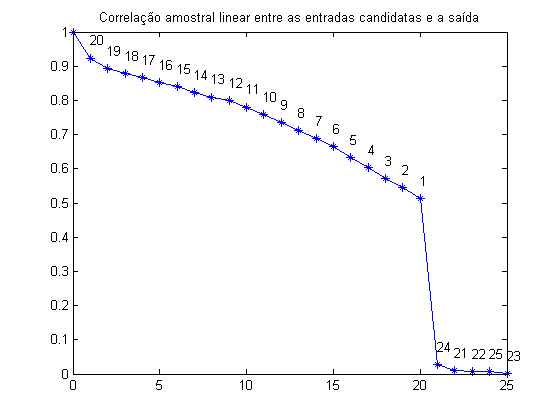
\includegraphics[width=1\linewidth]{image/filtro_lin}
					  \caption{Resultado do \textit{filtro linear}.}
					  \label{fig:filtro_lin}
					\end{subfigure}%
					\begin{subfigure}{.5\textwidth}
					  \centering
					  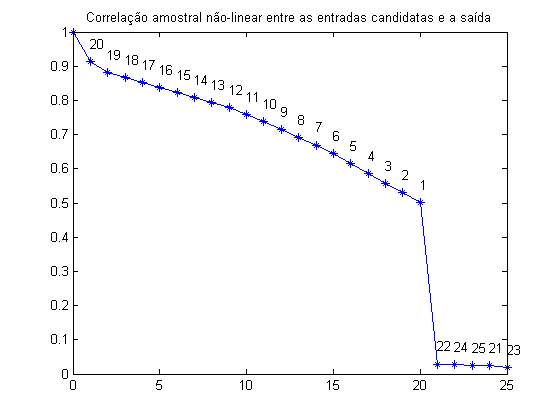
\includegraphics[width=1\linewidth]{image/filtro_nlin}
					  \caption{Resultado do \textit{filtro não linear}.}
					  \label{fig:filtro_nlin}
				\end{subfigure}
				
				\caption{Resultados das execuções das funções de filtro.}
				\end{figure}
				
				
			\FloatBarrier
				
			Conclui-se portanto que as variáveis de \(1\) a \(20\) apresentam as maiores
			correlações, tanto a linear \(R_{linear}\) quanto a não linear \(R_{nlinear}\),
			em relação à saída, sendo a \(20^a\) a mais correlata. A ordem de relevância em
			que elas aparecem também é a mesma, isto é, a sêquencia decrescente de 20 até 1
			é observada em ambos os casos, e a maior diferença percentual entre
			\(R_{linear}\) e \(R_{nlinear}\) é de \(3.12\%\), correspondente à \(13^a\)
			variável.
				
				\vspace{12pt}
				
			Observa-se ainda que as variáveis 21 até 25 apresentam \(R_{linear}\) e
			\(R_{nlinear}\) muito inferiores em relação aos valores das outras varíaveis
			e que a sua ordem de relevância é diferente: para o filtro \textit{linear} temos
			a sequência 24, 21, 22, 25 e 23, enquanto que para o \textit{não linear} obtemos
			22, 24, 25, 21 e 23.
			
			
			\item 
			\label{item:forwsunspot}
			Para o método \textbf{\textit{forward selection}} \footnote{As
			imagens referentes a estas execuções encontram-se na figura \ref{fig:forw}
			na seção \textbf{Anexos} no fim do documento}, obtem-se para as 5 execuções os seguintes dados:
			
			\begin{table}[H]
				    \centering
				    \footnotesize
					\caption{\label{tab:forward1_sunspot} Resultados da execução
					\textit{\textbf{1}}.}
				    \vspace{-6pt}
					\begin{tabular}{|c | c | c | c | c | c | c | c | c | c | c | c | c | c|}
					\hline
					Entradas & 20 & 18 & 17 & 3 & 12 & 19 & 15 & 1 & 16 & 11 & 23 & 5 & 7 \\
					\hline
					Erro mínimo & \multicolumn{13}{c|}{\(1.1765\)}  \\ \hline
					No. de Variáveis & \multicolumn{13}{c|}{\(13\)}  \\
					\hline
					
					\end{tabular}	    
			    \end{table}    

		\vspace{-12pt}

			\begin{table}[H]
				    \centering
					\caption{\label{tab:forward2_sunspot} Resultados da execução
					\textit{\textbf{2}}.}
					\footnotesize
				    \vspace{-6pt}
					\begin{tabular}{|c | c | c | c | c | c | c | c | c | c | c | c | c | c | c |
					c|}
					\hline
					Entradas & 20 & 18 & 17 & 3 & 12 & 19 & 15 & 1 & 10 & 5 & 22 & 7 & 21 & 25 & 16 \\
					\hline
					Erro mínimo & \multicolumn{15}{c|}{\(1.1745\)}  \\ \hline
					No. de Variáveis & \multicolumn{15}{c|}{\(15\)}  \\
					\hline
					
					\end{tabular}	    
			    \end{table}     

		\vspace{-12pt}

			\begin{table}[H]
				    \centering
				    \footnotesize
					\caption{\label{tab:forward3_sunspot} Resultados da execução
					\textit{\textbf{3}}.}
				    \vspace{-6pt}
					\begin{tabular}{|c | c | c | c | c | c | c | c | c | c | c | c | c | c | c|}
					\hline
					Entradas & 20 & 18 & 17 & 3 & 12 & 15 & 19 & 1 & 16 & 23 & 5 & 10 & 13 & 24 \\
					\hline
					Erro mínimo & \multicolumn{14}{c|}{\(1.1727\)}  \\ \hline
					No. de Variáveis & \multicolumn{14}{c|}{\(14\)}  \\
					\hline
					
					\end{tabular}	    
			    \end{table}     

		\vspace{-12pt}

			\begin{table}[H]
				    \centering
				    \footnotesize
					\caption{\label{tab:forward4_sunspot} Resultados da execução
					\textit{\textbf{4}}.}
				    \vspace{-6pt}
					\begin{tabular}{|c | c | c | c | c | c | c | c | c | c | c | c | c | c | c
					| c|}
					\hline
					Entradas & 20 & 18 & 17 & 3 & 12 & 15 & 19 & 1 & 16 & 10 & 5 & 23 & 24 & 13 & 21 \\
					\hline
					Erro mínimo & \multicolumn{15}{c|}{\(1.1707\)}  \\ \hline
					No. de Variáveis & \multicolumn{15}{c|}{\(15\)}  \\
					\hline
					
					\end{tabular}	    
			    \end{table} 
			    
		\vspace{-12pt}

			\begin{table}[H]
				    \centering
				    \footnotesize
					\caption{\label{tab:forward5_sunspot} Resultados da execução
					\textit{\textbf{5}}.}
				    \vspace{-6pt}
					\begin{tabular}{|c | c | c | c | c | c | c | c | c | c | c | c | c|}
					\hline
					Entradas & 20 & 18 & 17 & 3 & 12 & 19 & 15 & 1 & 10 & 11 & 5 & 7 \\
					\hline
					Erro mínimo & \multicolumn{12}{c|}{\(1.1768\)}  \\ \hline
					No. de Variáveis & \multicolumn{12}{c|}{\(12\)}  \\
					\hline
					
					\end{tabular}	    
			    \end{table} 
	
			    \FloatBarrier
	
		Considerando somente as primeiras cinco variáveis selecionadas em cada execução,
		percebe-se que, em realidade, elas são todas iguais: 20, 18, 17, 3 e 12, nessa
		sequência. Na sexta posição, encontra-se a variável 19 (3 ocasiões) ou a 15 (2
		ocasiões) e na sétima, a variável 1. À partir dessa posição, as entradas
		selecionadas variam a cada iteração.
		
		\vspace{12pt}	
	
		Para o método \textbf{\textit{backward elimination}}\footnote{As
			imagens referentes a estas execuções encontram-se na figura \ref{fig:back}
			na seção \textbf{Anexos} no fim do documento}, obtem-se:
			
			\begin{table}[H]
				    \centering
				    \footnotesize
					\caption{\label{tab:backward1_sunspot} Resultados da execução
					\textit{\textbf{1}}.}
				    \vspace{-6pt}
					\begin{tabular}{|c | c | c | c | c | c | c | c | c | c | c | c | c | c | c |
					c|}
					\hline
					Entradas & 23 & 25 & 24 & 5 & 22 & 16 & 21 & 1 & 18 & 15 & 19 & 12 & 3 & 17 & 20  \\
					\hline
					Erro mínimo & \multicolumn{15}{c|}{\(1.1711\)}  \\ \hline
					No. variáveis restantes & \multicolumn{15}{c|}{\(15\)}  \\
					\hline
					
					\end{tabular}	    
			    \end{table}    

		\vspace{-12pt}

			\begin{table}[H]
				    \centering
				    \footnotesize
					\caption{\label{tab:backward2_sunspot} Resultados da execução
					\textit{\textbf{2}}.}
				    \vspace{-6pt}
					\begin{tabular}{|c | c | c | c | c | c | c | c | c | c | c | c | c | c | c
					|}
					\hline
					Entradas & 8 & 25 & 11 & 7 & 5 & 16 & 1 & 15 & 18 & 19 & 12 & 3 & 17 & 20  \\
					\hline
					Erro mínimo & \multicolumn{14}{c|}{\(1.1717\)}  \\ \hline
					No. variáveis restantes & \multicolumn{14}{c|}{\(14\)}  \\
					\hline
					
					\end{tabular}	    
			    \end{table}       

		\vspace{-12pt}

			\begin{table}[H]
				    \centering
				    \footnotesize
					\caption{\label{tab:backward3_sunspot} Resultados da execução
					\textit{\textbf{3}}.}
				    \vspace{-6pt}
					\begin{tabular}{|c | c | c | c | c | c | c | c | c | c | c | c | c | c | c |
					c |}
					\hline
					Entradas & 8 & 7 & 23 & 21 & 5 & 16 & 11 & 1 & 18 & 15 & 19 & 12 & 3 & 17 & 20  \\
					\hline
					Erro mínimo & \multicolumn{15}{c|}{\(1.1744\)}  \\ \hline
					No. variáveis restantes & \multicolumn{15}{c|}{\(15\)}  \\
					\hline
					
					\end{tabular}	    
			    \end{table}       
		\vspace{-12pt}

			\begin{table}[H]
				    \centering
				    \footnotesize
					\caption{\label{tab:backward4_sunspot} Resultados da execução
					\textit{\textbf{4}}.}
				    \vspace{-6pt}
					\begin{tabular}{|c | c | c | c | c | c | c | c | c | c  | c | c | c | c | c
					| c | c | }
					\hline
					Entradas & 6 & 21 & 7 & 8 & 10 & 24 & 16 & 25 & 1 & 18 & 15 & 19 & 12 & 3 & 17 & 20  \\
					\hline
					Erro mínimo & \multicolumn{16}{c|}{\(1.1733\)}  \\ \hline
					No. variáveis restantes & \multicolumn{16}{c|}{\(16\)}  \\
					\hline
					
					\end{tabular}	    
			    \end{table}  	
			    
		\vspace{-12pt}

			\begin{table}[H]
				    \centering
				    \footnotesize
					\caption{\label{tab:backward5_sunspot} Resultados da execução
					\textit{\textbf{5}}.}
				    \vspace{-6pt}
					\begin{tabular}{|c | c | c | c | c | c | c | c | c | c | c | c | c | c | c|}
					\hline
					Entradas & 7 & 21 & 13 & 16 & 5 & 10 & 1 & 18 & 15 & 19 & 3 & 12 & 17 & 20   \\
					\hline
					Erro mínimo & \multicolumn{14}{c|}{\(1.1748\)}  \\ \hline
					No. variáveis restantes & \multicolumn{14}{c|}{\(14\)}  \\
					\hline
					
					\end{tabular}	    
			    \end{table}  	
	
			    \FloatBarrier	
	
		Observa-se que o número de variáveis restantes para as execuções do
		\textit{backward elimination} é ligeiramente superior em relação ao método
		anterior, apresentando uma média de 15 variáveis escolhidas contra
		aproximadamente 14 do \textit{forward selection}. A média do erro quadrado
		médio na construção do modelo é inferior para \textit{backward
		elimination}: 1.1731 contra 1.1742. Nota-se ainda que algumas variáveis foram
		escolhidas em todas as execuções de ambos, sendo elas, por exemplo, a 20, 17,
		3, 12 e a 15.
	
		 \item Entradas que possuem as maiores correlações não são as primeiras a
		 serem adicionadas ao modelo pela presença de \textit{redundância} entre elas.
		 Se uma variável é altamente correlata com uma outra, eu não precisaria, em
		 príncipio, conhecer as duas, já que a partir de um única, eu sou capaz de
		 determinar a outra. Em outras palavras, variáveis \textit{redundantes}
		 adicionam pouca informação ao sistema. Por exemplo, a correlação entre as
		 variáveis 20 e 19 do arquivo \texttt{dados1.mat} vale 0.9239 (valor obtido
		 pelo comando \texttt{corr(X(:,20), X(:,19))} do MATLAB). Isso signfica que se
		 \(X_{20}\) é alto, então \(X_{19}\) também o é e, portanto, nenhuma outra
		 informação é adicionada ao modelo. É por essa razão que nas execuções acima,	
		 \(X_{20}\) é escolhida inicialmente e \(X_{19}\), só depois de algumas
		 iterações.
		 
		\item Variáveis de baixa correlação com a saída podem proporcionar um grande poder
		de separação, se consideradas juntamente com outras\footnote{No artigo \textit {[ Guyon,  I.;  Elisseeff,  A.
		“An  introduction  to  variable  and feature selection”, Journal of Machine
		Learning Resear ch, vol. 3, pp. 1157 - 1182 2003 ]}, o autor dá um exemplo dessa
		afirmação na seção 3.3.}. Desta maneira, as variáveis de menor correlação são
		separadas mais facilmente em relação àquelas de maior correlação, permitindo
		assim a detecção de classes com maior precisão. Em outras palavras, entradas
		mais próximas das variáveis de baixa correlação podem ser classificadas mais
		facilmente.

		 \item As variáveis geradas aleatoriamente (\( X_{21} \cdots X_{25} \))
		 apresentam correlações em relação à saída praticamente nulas (os resultados
		 de \texttt{corr (X(:,21), S)} \ldots  ~\texttt{corr (X(:,25), S)} estão
		 mostrados na tabela \ref{tab:corr.aleat.}). Dessa maneira, elas são
		 escolhidas em ambos os modelos pelos mesmos motivos daqueles discutidos nos
		 dois itens anteriores (\textit{redundância} e \textit{poder de separação}).
		 
		 \begin{table}[H]
				    \centering
					\caption{\label{tab:corr.aleat.} Correlação das variáveis
					aleatórias execução 1 do \textit{forward selection}.}
					\begin{tabular}{| c | c |}
					
					\hline
					Variável \(X_i \) & \texttt{corr (X(:,i), S)} \\ \hline \hline
					\(X_{21}\) & 0.001347309212350 \\ \hline
					\(X_{22}\) & 0.011839959350690 \\ \hline
					\(X_{23}\) & -0.037287334573179 \\ \hline
					\(X_{24}\) & -0.007005116183944 \\ \hline
					\(X_{25}\) & 0.001963170472808 \\ \hline
					
					
					\end{tabular}	    
			    \end{table}  	
	
			    \FloatBarrier
		 
		\end{enumerate}
		
		\item \begin{enumerate}
		  \item O arquivo \texttt{wineq.mat} é composto por duas estruturas de dados.
		  A primeira, matriz \(X_{1593 \times 11}\), possui 11 colunas, correpondentes
		  a cada uma das variáveis de entrada, e 1593 linhas, simbolizando 1593 dados
		  disponíveis. De acordo com o \textit{website} de onde tais dados foram
		  retirados, essas variáveis correspondem a diversas propriedades que podem
		  ser extraídas de um vinho, sendo elas \textit{fixed acidity},
		  \textit{volatile acidity}, \textit{citric acid}, \textit{residual sugar},
		  \textit{chlorides}, \textit{free sulfur dioxide}, \textit{total sulfur
		  dioxide}, \textit{density}, \textit{pH}, \textit{sulphates} e
		  \textit{alcohol}. Foram considerados variações de vinhos tintos e brancos do
		  vinho português \textit{Vinho Verde}. A tabela abaixo mostra algumas
		  características dessas propriedades.
		  
		  \begin{table}[H]
			    \centering
				\footnotesize
				\caption{\label{tab:wineq.mat} Informações correpondentes às variáveis de
				\texttt{wineq.mat}.}
				\begin{tabular}{| c | c |  c | c | c |}
				
				\hline
				Variável & Média & Max. & Min. & \textit{Standard Deviation} \\ \hhline{|=|=|=|=|=|} 
				\textit{fixed acidity} & 0.52324 & 1 & 0.28931 &
				0.10932 \\ \hline \textit{volatile acidity} & 0.33385 & 1 & 0.075949 & 0.11333 \\ \hline
				 \textit{citric acid} & 0.27116 & 1 & 0 & 0.19495 \\ \hline
				 \textit{residual sugar} & 0.16374 & 1 & 0.058065 & 0.090957 \\ \hline
				 \textit{chlorides} & 0.14321 & 1 & 0.01964 & 0.077153 \\ \hline
				 \textit{free sulfur dioxide} & 0.2205 & 1 & 0.013889 & 0.14537 \\ \hline
				 \textit{total sulfur dioxide}& 0.16052 & 1 & 0.020761 & 0.11379 \\ \hline
				 \textit{density} & 0.022051 & 1 & 0.0098643 & 0.096464 \\ \hline
				  \textit{pH} & 0.82574 & 1 & 0.68329 & 0.038451 \\ \hline
				 \textit{sulphates}& 0.32903 & 1 & 0.165 & 0.084846 \\ \hline
				 \textit{alcohol} & 0.69949 & 1 & 0.56376 & 0.071404 \\ \hline
				
				\end{tabular}	    
		    \end{table} 
		    
		    Para a saída, que mede o nível de qualidade de cada vinho, baseado em um
		    teste sensitivo, encontra-se:
		    
		    \begin{table}[H]
			    \centering
				\caption{\label{tab:wineqSaida.mat} Informações correpondentes à saída
				de
				\texttt{wineq.mat}.}
				\begin{tabular}{| c | c |  c | c | c |}
				
				\hline
				Variável & Média & Max. & Min. & \textit{Standard Deviation} \\ \hhline{|=|=|=|=|=|} 
				Saída & 0.70425 & 1 & 0.375 & 0.10101 \\ \hline
				
				\end{tabular}	    
		    \end{table} 
		    
		    \item As execuções de \texttt{filtro\_lin('dados2.mat')} e
		    \texttt{filtro\_nlin('dados2.mat')} são mostradas na figuras
		    \ref{fig:filtro_lin2} e \ref{fig:filtro_nlin2} a seguir.
		    
		    \begin{figure}[H]
				
				\centering
				
					\begin{subfigure}{.5\textwidth}
					  \centering
					  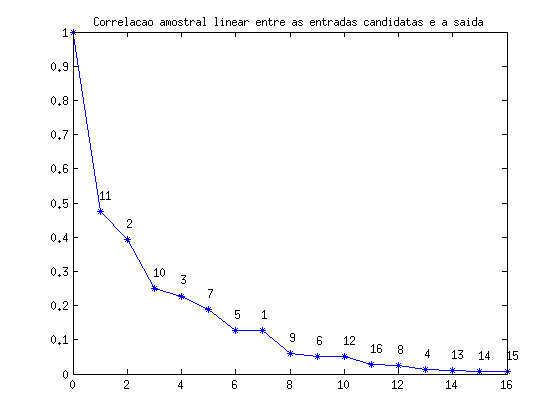
\includegraphics[width=1\linewidth]{image/filtro_lin2}
					  \caption{Resultado do \textit{filtro linear}.}
					  \label{fig:filtro_lin2}
					\end{subfigure}%
					\begin{subfigure}{.5\textwidth}
					  \centering
					  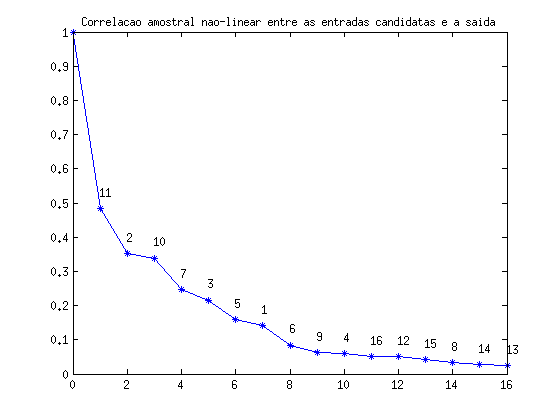
\includegraphics[width=1\linewidth]{image/filtro_nlin2}
					  \caption{Resultado do \textit{filtro não linear}.}
					  \label{fig:filtro_nlin2}
				\end{subfigure}
				
				\caption{Resultados das execuções das funções de filtro.}
				\end{figure}
				
			\FloatBarrier
			
			Neste caso, observa-se uma maior diferença entre as filtragens linear e não
			linear em relação ao estudo de caso anterior. Percebe-se inicialmente que a
			correlação da variável mais correlata (\(<0.5\)) aqui é muito inferior
			àquela mais correlata (\(>0.9\)) para os dados referentes aos
			\textit{Sunspots}. 
			
			\vspace{12pt}
			
			A ordem decrescente de correlação em que as variáveis aparecem também muda do
			caso linear para o não linear. A tabela seguinte evidencia
			esta afirmação. \(\Delta =  \frac {\left( R_{nlin} - R_{lin}
			\right)}{R_{nlin}} \), onde \(R\) é o valor da correlação linear ou não
			linear, representa a variação percentual entre as respectivas correlações.
			
			\begin{table}[H]
			    \centering
			    \footnotesize
				\caption{\label{tab:ordem} Ordens de aparição das variáveis.}
				\begin{tabular}{| c | c |  c | c | c | c | c |  c | c | c | c | c |  c | c |
				c | c | c |}
				\hline
				 & \multicolumn{16}{|c|}{Ordem} \\
				\hhline{|=|=|=|=|=|=|=|=|=|=|=|=|=|=|=|=|=|} 
				Linear & 11 & 2 & 10 & 3 & 7 & 5 & 1 & 9 & 6 & 12 &
				16 & 8 & 4 & 13 & 14 & 15 \\ \hline 
				
				\textit{Não} linear &  11 & 2 & 10 & 7 & 3 & 5 & 1 & 6 & 9 & 4 
				& 16 & 12 & 15 & 8 & 14 & 13 \\ \hline 
				
				\(\Delta\) & 0.01 & -0.12 & 0.26 & 0.07 & 0.13 & 0.2 &
				0.11 & 0.31 & 0.18 & 0.16 & 0.46 & 0.5 & 0.68 & 0.73 & 0.75 & 0.72 \\
				\hline
				\end{tabular}	    
		    \end{table} 

			
			\FloatBarrier
			
			Observa-se que a ordem muda sobretudo no fim da sequência, onde as
			variações percentuais são superiores.
			
			\item 
			\label{item:forwwineq}
			Para o método \textbf{\textit{forward selection}}\footnote{As
			imagens referentes a estas execuções encontram-se na figura \ref{fig:forw2}
			na seção \textbf{Anexos} no fim do documento}, obtem-se para as 5
			execuções os seguintes dados:
			
			\begin{table}[H]
					\setlength\tabcolsep{4pt}
					\begin{minipage}{0.48\textwidth}
					    \centering
					    \footnotesize
						\caption{\label{tab:forward1_wine} Resultados da execução
						\textit{\textbf{1}}.}
					    \vspace{-6pt}
						\begin{tabular}{|c | c | c | c | c | c | c | c | c |}
						\hline
						Entradas & 11 & 2 & 10 & 7 & 5 & 9 & 6 & 16 \\
						\hline
						Erro mínimo & \multicolumn{8}{c|}{\(1.0484\)}  \\ \hline
						No. de Variáveis & \multicolumn{8}{c|}{\(8\)}  \\
						\hline
						
						\end{tabular}
					\end{minipage}	    
					\begin{minipage}{0.48\textwidth}
					    \centering
						\caption{\label{tab:forward2_wine} Resultados da execução
						\textit{\textbf{2}}.}
						\footnotesize
					    \vspace{-6pt}
						\begin{tabular}{|c | c | c | c | c | c | c | c | c | c |}
						\hline
						Entradas & 11 & 2 & 10 & 7 & 5 & 9 & 6 & 13 & 14 \\
						\hline
						Erro mínimo & \multicolumn{9}{c|}{\(1.0491\)}  \\ \hline
						No. de Variáveis & \multicolumn{9}{c|}{\(9\)}  \\
						\hline
						
						\end{tabular}	
					\end{minipage}	    
			    \end{table}     

		\vspace{-12pt}

			\begin{table}[H]
					\setlength\tabcolsep{4pt}
					\begin{minipage}{0.48\textwidth}
					    \centering
					    \footnotesize
						\caption{\label{tab:forward3_wine} Resultados da execução
						\textit{\textbf{3}}.}
					    \vspace{-6pt}
						\begin{tabular}{|c | c | c | c | c | c | c | c | c |}
						\hline
						Entradas & 11 & 2 & 10 & 7 & 5 & 9 & 6 & 13 \\
						\hline
						Erro mínimo & \multicolumn{8}{c|}{\(1.0495\)}  \\ \hline
						No. de Variáveis & \multicolumn{8}{c|}{\(8\)}  \\
						\hline
						
						\end{tabular}	    
					\end{minipage}	    
					\begin{minipage}{0.48\textwidth}
					    \centering
					    \footnotesize
						\caption{\label{tab:forward4_wine} Resultados da execução
						\textit{\textbf{4}}.}
					    \vspace{-6pt}
						\begin{tabular}{|c | c | c | c | c | c | c | c | c|}
						\hline
						Entradas & 11 & 2 & 10 & 7 & 5 & 9 & 6 & 14 \\
						\hline
						Erro mínimo & \multicolumn{8}{c|}{\(1.0509\)}  \\ \hline
						No. de Variáveis & \multicolumn{8}{c|}{\(8\)}  \\
						\hline
						
						\end{tabular}
					\end{minipage}	    
			    \end{table} 
			    
			\vspace{-12pt}

			\begin{table}[H]
				    \centering
				    \footnotesize
					\caption{\label{tab:forward5_wine} Resultados da execução
					\textit{\textbf{5}}.}
				    \vspace{-6pt}
					\begin{tabular}{|c | c | c | c | c | c | c | c | c|}
					\hline
					Entradas & 11 & 2 & 10 & 7 & 5 & 9 & 6 & 13 \\
					\hline
					Erro mínimo & \multicolumn{8}{c|}{\(1.0509\)}  \\ \hline
					No. de Variáveis & \multicolumn{8}{c|}{\(8\)}  \\
					\hline
					
					\end{tabular}	    
			    \end{table} 
	
			    \FloatBarrier
			    
			Para o método \textbf{\textit{backward elimination}}\footnote{As
			imagens referentes a estas execuções encontram-se na figura \ref{fig:back2}
			na seção \textbf{Anexos} no fim do documento}, obtem-se:
			
			\begin{table}[H]
					\setlength\tabcolsep{4pt}
					\begin{minipage}{0.48\textwidth}
					    \centering
					    \footnotesize
						\caption{\label{tab:backward1_wine} Resultados da execução
						\textit{\textbf{1}}.}
					    \vspace{-6pt}
						\begin{tabular}{|c | c | c | c | c | c | c | c | c |}
						\hline
						Entradas & 13 & 6 & 9 & 5 & 7 & 10 & 2 & 11 \\
						\hline
						Erro mínimo & \multicolumn{8}{c|}{\(1.0496\)}  \\ \hline
						No. de Variáveis & \multicolumn{8}{c|}{\(8\)}  \\
						\hline
						
						\end{tabular}
					\end{minipage}	    
					\begin{minipage}{0.48\textwidth}
					    \centering
						\caption{\label{tab:backward2_wine} Resultados da execução
						\textit{\textbf{2}}.}
						\footnotesize
					    \vspace{-6pt}
						\begin{tabular}{|c | c | c | c | c | c | c | c | c | c |}
						\hline
						Entradas & 15 & 3 & 14 & 9 & 5 & 7 & 10 & 2 & 11  \\
						\hline
						Erro mínimo & \multicolumn{9}{c|}{\(1.0558\)}  \\ \hline
						No. de Variáveis & \multicolumn{9}{c|}{\(9\)}  \\
						\hline
						
						\end{tabular}	
					\end{minipage}	    
			    \end{table}     

		\vspace{-12pt}

			\begin{table}[H]
					\setlength\tabcolsep{4pt}
					\begin{minipage}{0.48\textwidth}
					    \centering
					    \footnotesize
						\caption{\label{tab:backward3_wine} Resultados da execução
						\textit{\textbf{3}}.}
					    \vspace{-6pt}
						\begin{tabular}{|c | c | c | c | c | c | c | c | c | c | c |}
						\hline
						Entradas & 15 & 12 & 3 & 6 & 9 & 5 & 7 & 10 & 2 & 11  \\
						\hline
						Erro mínimo & \multicolumn{10}{c|}{\(1.0532\)}  \\ \hline
						No. de Variáveis & \multicolumn{10}{c|}{\(10\)}  \\
						\hline
						
						\end{tabular}	    
					\end{minipage}	    
					\begin{minipage}{0.48\textwidth}
					    \centering
					    \footnotesize
						\caption{\label{tab:backward4_wine} Resultados da execução
						\textit{\textbf{4}}.}
					    \vspace{-6pt}
						\begin{tabular}{|c | c | c | c | c | c | c | c | c| c| c|}
						\hline
						Entradas & 3 & 1 & 14 & 6 & 9 & 5 & 7 & 10 & 2 & 11 \\
						\hline
						Erro mínimo & \multicolumn{10}{c|}{\(1.0548\)}  \\ \hline
						No. de Variáveis & \multicolumn{10}{c|}{\(10\)}  \\
						\hline
						
						\end{tabular}
					\end{minipage}	    
			    \end{table} 
			    
			\vspace{-12pt}

			\begin{table}[H]
				    \centering
				    \footnotesize
					\caption{\label{tab:backward5_wine} Resultados da execução
					\textit{\textbf{5}}.}
				    \vspace{-6pt}
					\begin{tabular}{|c | c | c | c | c | c | c | c | c| c|}
					\hline
					Entradas & 12 & 6 & 14 & 9 & 5 & 7 & 10 & 2 & 11 \\
					\hline
					Erro mínimo & \multicolumn{9}{c|}{\(1.0497\)}  \\ \hline
					No. de Variáveis & \multicolumn{9}{c|}{\(9\)}  \\
					\hline
					
					\end{tabular}	    
			    \end{table} 
	
			    \FloatBarrier
		     
		     Observa-se que para a técnica de \textit{forward selection} as primeiras
		     sete entradas selecionadas foram as mesmas para as 5 execuções, sendo
		     elas a 11, 2, 10, 7, 5, 9 e 6. As restantes escolhidas fazem parte das
		     entradas aleatórias, calculadas para cada execução. Em média, foram
		     escolhidas 8 variáveis e produziu-se um erro de 1.04976.
		     
		     \vspace{12pt}
		     
		     Em relação à técnica de \textit{backward elimination}, as mesmas
		     variáveis citadas no parágrafo anterior estiveram presentes, com exceção
		     da 6, que esteve ausente somente na execução 2. Foram selecionadas, em
		     média, um número maior de variáveis, 9, e um erro superior, 1.05262. As
		     variáveis restantes foram escolhidas dentre as geradas aleatoriamente.
		     
		     \vspace{12pt}
		     
		     Finalmente, as váriaveis que foram escolhidas nos primeiros lugares na
		     \textit{forward selection} seriam eliminadas por último na
		     \textit{backward elimination}, confirmando assim um certo nível de
		     semelhância nos resultados das duas técnicas.
		     
		\end{enumerate}
\end{enumerate}
		  
